\begin{figure}[!ht]
\vspace{3mm}
\begin{center}
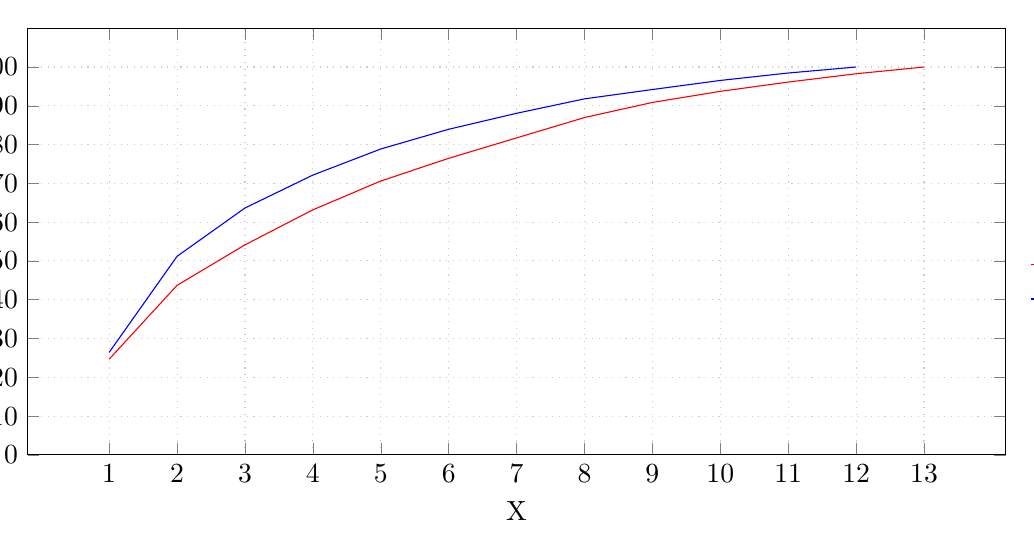
\begin{tikzpicture}[trim axis left, trim axis right]
	\begin{axis}[
		xlabel=X,
		ylabel=Y,
		xtick={1,...,13},
		ymin=0,
		ytick={0,10,...,100},
		legend style={
			at={(1,0.5)},
			xshift=0.2cm,
			anchor=north west,
			nodes=right,
			draw=none
		},
		grid=major,
   		grid style={dotted,lightgray!80!white},
		%axis lines=left
		width=14cm,
		height=7cm,
	]
	\addplot[color=red] coordinates{
		(1,24.6718)
		(2,43.7092)
		(3,54.14785132)
		(4,63.1821339)
		(5,70.60866985)
		(6,76.45681086)
		(7,81.7263871)
		(8,86.97406846)
		(9,90.86684525)
		(10,93.72329021)
		(11,96.11621437)
		(12,98.25885879)
		(13,100)		
	};
	\addplot[color=blue] coordinates{
		(1,26.42529337)
		(2,51.19458535)
		(3,63.64859236)
		(4,72.13773673)
		(5,78.8676646)
		(6,83.94694845)
		(7,88.06842906)
		(8,91.7882484)
		(9,94.19470806)
		(10,96.53607266)
		(11,98.45170481)
		(12,100)
		
	};
	\legend{Testa,Testb}
	\end{axis}
\end{tikzpicture}
\end{center}
\vspace{-3mm}
\caption{test1}
\label{fig.test1}
\vspace{3mm}
\end{figure}

\begin{figure}[ht]
\centering
\begin{tikzpicture}
\begin{axis}[
xlabel={Zeit},
ylabel={Position},
ymin=0,
ymax=6,
width=100mm,
height=80mm,
ytick={0,1,...,5},
legend style={at={(1,1)},	anchor=north east, xshift=-1mm,	yshift=-1mm}
]
\pgfplotstableread{plot/test.txt}\datatable
\addplot[color=red,mark=square*] table[x index=0,y index=1] from \datatable;
%\addplot[no markers] table[x index=0,y index=3] from \datatable;
%\addplot[no markers] table[y = Leistung] {plot/test.txt}  ;
\legend{test}
\end{axis}
\end{tikzpicture}
\caption{test2}
\label{fig.test2}
\end{figure}

\begin{figure}
\begin{center}
\begin{tikzpicture}[trim axis left, trim axis right]
  \begin{axis}[
    	ytick={0,0.1,...,1.1},
    		minor y tick num=5,
    		ymax=1.1,
    		ylabel=Y-Achse,
    		xtick={1,...,4},
    		x tick label style={align=center},
    		xticklabels={A, B},
    		boxplot/draw direction=y,
    		width=8cm,
    		height=8cm,
    		thick,
    ]
%    \addplot+[color=red,mark=x,
%    		boxplot prepared={
%      		lower whisker=,
%      		lower quartile=,
%      		median=,
%      		upper quartile=,
%      		upper whisker=
%    		},
%    ] %coordinates {};
%    table[row sep=\\,y index=0] {0.7054\\ 0.9773\\  0.9763\\ 0.9698\\ 0.7118\\ 0.6919\\ 0.9727\\ 0.7006\\ 0.974\\ 0.7077\\}; %Ausreisser
    \addplot+[color=Green,mark=x,
    		boxplot prepared={
      		median=0.3036,
      		upper quartile=0.34925,
      		lower quartile=0.2674,
      		upper whisker=0.5597,
      		lower whisker=0.18718
		},
    ] %coordinates {};
    table[row sep=\\,y index=0] {0.6045\\ 0.1818\\ 0.5826\\ 0.5688\\ 0.1814\\ 0.1825\\ 0.5750\\ 0.1783\\ 0.6312\\ 0.1793\\}; %Ausreisser
  \end{axis}
\end{tikzpicture}
\caption{Box-Whisker-Plot}
\label{fig.error_boxplot}
\end{center}
\vspace{-3mm}
\end{figure}